\section{Magnetic Fields}

% Magnetic fields

We are interested in modeling the behaviour of the net magnetization,
$\textbf{M}$, of spin packets under the influence of one or more
magnetic fields. This is a function dependent on the time, $t$, and
position, $\textbf{p}$, within the sample. The functions describing
each coordinate component of $\textbf{M}$ are $M_x$, $M_y$ and
$M_z$. Thus our net magnetization is given by

\begin{displaymath}
  \textbf{M}(t, \textbf{p}) = \langle M_x(t, \textbf{p}), M_y(t, \textbf{p}), M_z(t, \textbf{p}) \rangle
\end{displaymath}

As stated previously, when only the static magnetic field
$\mathbf{B}_0 = \langle 0, 0, B_0 \rangle$ is active, $\textbf{M}$
will lie at equilibrium along the z-axis. Thus $\textbf{M} = \langle
0, 0, M_{eq} \rangle$, where $M_{eq}$ is the magnitude of $\textbf{M}$.

The gyromagnetic ratio, $\gamma$, of a particle is the ratio of it's
magnetic dipole moment to it's angular momentum. This means that
$\gamma$ can tell us how fast the net magnetization will precess
around the magnetic field applied to it. 

\begin{displaymath}
  \omega = \gamma \| \mathbf{B} \|
\end{displaymath}

The gyromagnetic ratio for hydrogen atoms is $42.58 \cdot 10^6 Hz / T$
(hertz pr. tesla).

With this we can now formulate the bloch equations that descripe the
net magnetizations rate of change over time with respect to the sum of
magnetic fields, $\mathbf{B}$.

% Bloch equations
\begin{displaymath}
  \frac{d\mathbf{M}}{dt} = \gamma \mathbf{M} \times \mathbf{B} -
  \frac{\langle M_x, M_y, 0 \rangle}{T_2} - \frac{\langle 0, 0, M_z -
    M_{eq} \rangle}{T_1}
\end{displaymath}

$T_1$ and $T_2$ are relaxation times for the spins. $T_1$ is the
\textit{spin-lattice} relaxation time and describe how fast the net
magnetization will return to equilibrium. $T_2$ is the
\textit{spin-spin} relaxation time and reflects how fast the magnitude
of the net magnetizations transverse components goes to 0. $T_2$ will
always be smaller or equal to $T_1$.

% @TODO figures of relaxation times

% Magnetic fields

As explained earlier $\mathbf{B}$ is the sum of three magnetic fields;
the static field $\mathbf{B}_0$, the RF field $\mathbf{B}_1$ and the
gradient field $\mathbf{B}_G$.

\begin{displaymath}
  \mathbf{B} = \mathbf{B}_0 + \mathbf{B}_1 + \mathbf{B}_G
\end{displaymath}

The static field, as written earlier, is simply $\mathbf{B}_0 =
\langle 0, 0, B_0 \rangle$, which is a magnetic field lying along the
z-axis. $\mathbf{B}_0$ causes the spin of the nuclei to precess about
the z-axis at frequency $\gamma B_0 = \omega_0$.

The RF magnetic field, or RF pulse, $\mathbf{B}_1$ is more complex. It
has to rotate the net magnetization into the transverse plane, while
the aggregate magnetic moment is precessing about the $\mathbf{B}_0$
field. In order to do that $\mathbf{B}_1$ is itself rotating about
$\mathbf{B}_0$ at frequence $\omega_0$.

\begin{displaymath}
  \mathbf{B}_1 = \langle B_1 cos(\omega_0 t), B_1 sin(\omega_0 t), 0\rangle
\end{displaymath}


\subsection{Magnetic gradients}

Recall from earlier that if all net magnetizations are spinning in the
same phase and at the same frequency, they are indistinguishable to
the fourier transform and thus produces on image with only one
voxel. We will now in more detail present the gradient fields that
help distinguish the individual spin packets.

We have previously included the gradient fields in our equations as
one variable, $\mathbf{B}_G$. This is purely done to simplify the
equations. In practice one must remember that the gradient field
actually consists of the 3 seperat gradient fields described in
\refsec{sec:MRI}.

\begin{displaymath}
  \mathbf{B}_G = \mathbf{B}_{G_s} + \mathbf{B}_{G_\phi} + \mathbf{B}_{G_f}
\end{displaymath}

As can be seen on \reffig{fig:gradientSequence} the individual
gradients are never active at the same time.

% Constant gradient field along the x axis (read-out direction). The
% strength of the gradient field increases along the x-axis and never
% changes over the course of the signal acquisition.

\begin{displaymath}
  \omega = \gamma (B_0 + x B_{G_f})
\end{displaymath}


% The y-axis is the phase encode direction and is phase encoded with a
% phase gradient.


\begin{figure}
  \centering
  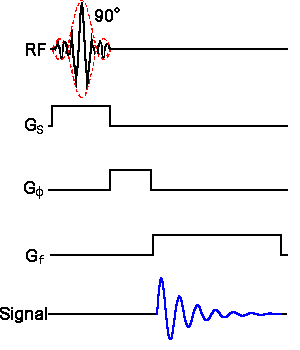
\includegraphics[width=5cm]{gradientSequence}
  \caption{A timing diagram of the application of gradients with
    respect to the RF pulse and signal acquisition.}
  \label{fig:gradientSequence}
\end{figure}


With only the static magnetic field $\mathbf{B}_0$ and
$\mathbf{B}_{G_f} = \langle 0, 0, p_x * B_{G_f} \rangle$ active, the
block equations simply to

% Bloch equations with the gradient and B0, which is what we're
% solving

\begin{displaymath}
  \begin{array}{l}
    \frac{dM_x}{dt} = \gamma (B_0 + p_x * B_{G_f}) M_y - \frac{M_x}{T_2} \\
    \frac{dM_y}{dt} = - \gamma (B_0 + p_x * B_{G_f}) M_x - \frac{M_y}{T_2} \\
    \frac{dM_z}{dt} = - \frac{M_z - M_{eq}}{T_1}
  \end{array}
\end{displaymath}



%%% Local Variables:
%%% mode: latex
%%% TeX-master: t
%%% TeX-PDF-mode: t
%%% End:
